\documentclass[tikz]{standalone}
\usepackage{pgfplots}

\begin{document}
    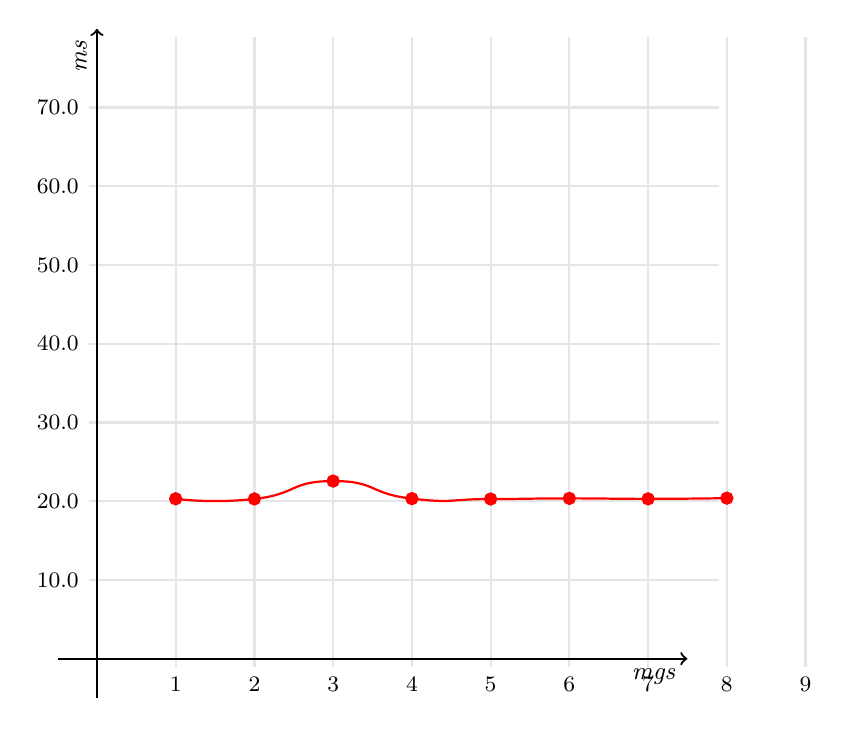
\begin{tikzpicture}[thick]

        \foreach \y in {1, 2, ..., 7} {
            \draw[gray!20] (-0.1, \y) node[left, black] {\footnotesize \pgfmathparse{\y*10}\pgfmathresult} -- ++ (8, 0);
        }
        
        
        \foreach \x in {1, 2, ..., 9}{
            \draw[gray!20] (\x, -0.1) node[below, black]{\footnotesize \x} -- ++ (0, 8);
        }

        \draw[->] (0, -0.5) -- ++ (0, 8.5) node[above left, rotate=90]{\small \textit{ms}};
        \draw[->] (-0.5, 0) -- ++ (8, 0) node[below left]{\small \textit{mgs}};
    
        \draw [red] plot [smooth, tension=1, mark=*] coordinates {(1, 2.031) (2, 2.029) (3, 2.256) (4, 2.033) (5, 2.028) (6, 2.036) (7, 2.03) (8, 2.039) };
    \end{tikzpicture}
\end{document}